\begin{figure}
    \centering
    \begin{small}
    \begin{sc}
    \begin{tikzpicture}[node distance=0.2cm, auto]
    
    \tikzstyle{header} = [text centered]
    \tikzstyle{pict} = [inner xsep=4px]
    \tikzstyle{arrow} = [thick,->,-{Latex[scale=1]}]
    

    % \node [pict, right=of input, label={[align=center]above:Edges}] (edge) {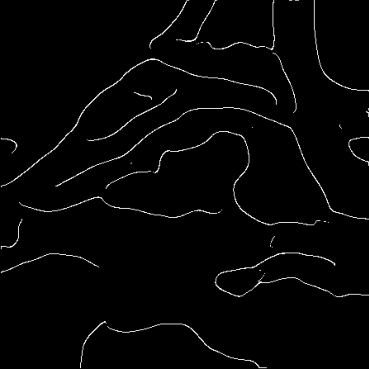
\includegraphics[width=2cm]{figures/edge/edges2.png}};
    \node [pict, label={[align=center]right:EDGE\\sampling}] (sample) {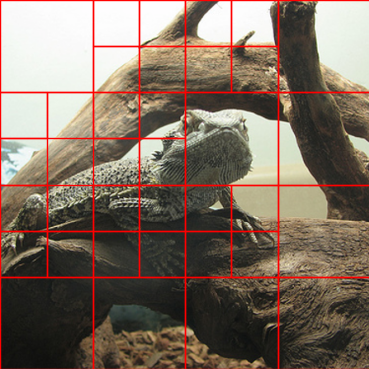
\includegraphics[width=1.8cm]{figures/edge/edges3.png}};

    \node [pict, above=of sample, label={[align=center]right:CENTRAL\\sampling}] (central) {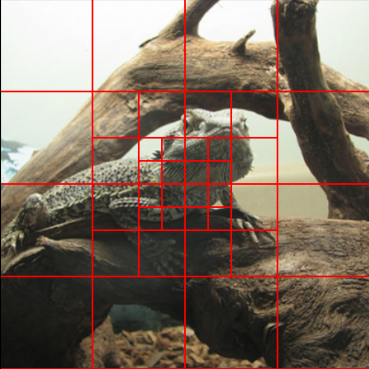
\includegraphics[width=1.8cm]{figures/edge/central.png}};


    \node[fit=(sample) (central) (central) (sample), fit margins={left=0cm,right=0cm,bottom=0cm,top=0cm}] (bbox) {};

    \node [pict, left=1cm of bbox, label={[align=center]left:Input}] (input) {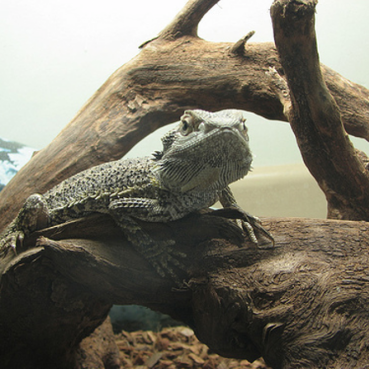
\includegraphics[width=1.8cm]{figures/edge/edges1.png}};

    \draw [arrow] (input) -- (sample);
    \draw [arrow] (input) -- (central);

    \end{tikzpicture}
    \end{sc}
    \end{small}
    % \afterplot
    \caption{\textbf{Patch sampling strategies:} We introduce two sampling strategies to show the benefits of elastic sampling. CENTRAL employ human retina-like higher density sampling in the center, EDGE samples based on weights provided by an edge detector (the more edges the denser sampling).}
    \label{fig:adaptive}
\end{figure}